\section{线性规划的表述}
\label{sec:lp-formulation}

来源不同的线性模型，怎样写成同一种形式，使后面的定理和计算只需要处理这一种形式？我们先看资源配置和网络流两个模型，它们的约束长得很不一样；然后规定标准型，并逐项说明改写时什么保持不变、什么发生了变化。

\paragraph{资源配置}
车间问题可以这样一般化。有$n$种产品和$m$种资源，产品$j$的产量是$x_j$，单位利润是$p_j$，每生产一单位消耗资源$i$的量是$A_{i,j}$，资源$i$的总量是$b_i$。最大利润的产量由下面的问题决定：
\begin{equation}
 \max_{\bm{x}\in\mathbb{R}^n}\ \bm{p}^\top\bm{x}
 \quad\text{s.t.}\quad \bm{A}\bm{x}\leq\bm{b},\quad \bm{x}\geq\bm{0}.
 \label{eq:lp-resource-general}
\end{equation}
向量之间的不等号表示逐分量成立，$\bm{x}\geq\bm{0}$就是每个分量非负。车间问题对应$n=m=2$，数据是
\begin{equation}
 \bm{A}=\begin{bmatrix}1&1\\2&1\end{bmatrix},\qquad
 \bm{b}=\begin{bmatrix}4\\6\end{bmatrix},\qquad
 \bm{p}=\begin{bmatrix}3\\2\end{bmatrix}.
 \label{eq:lp-workshop-inequality}
\end{equation}
第一行是工时，第二行是原料。

这个模型能写成线性形式，靠的是两条假设。一是比例：产量加倍，利润和消耗都加倍。二是可加：两种产品的利润和消耗直接相加，互不影响。如果批量大了原料打折，单位消耗就依赖产量，约束里会出现$x_1x_2$或$x_1^2$这样的项，模型就不再是线性的。

\begin{definition}[线性规划]
 \label{def:lp-program}
 在$\mathbb{R}^n$中，以一个线性函数为目标，在有限个线性等式和非严格线性不等式的约束下求最小值或最大值，这样的问题称为线性规划。
\end{definition}

定义只允许非严格不等式。若允许$x<2$这样的约束，在其上最大化$x$，上确界$2$就取不到，这正是第~\ref{chap:optimization}章区分过的“下确界未达到”。非严格不等式和等式都定义闭集，这类麻烦在线性规划里不会由约束的开边界引起。

\paragraph{网络流}
第二个模型的约束是等式。图~\ref{fig:lp-network-instance}是一个有$4$个节点、$5$条有向弧的网络，每条弧旁的数字是运送一单位货物的费用。节点$1$要运出$1$单位货物，节点$4$要收到$1$单位，节点$2,3$只中转。

\begin{BookInlineFigure}
 \centering
 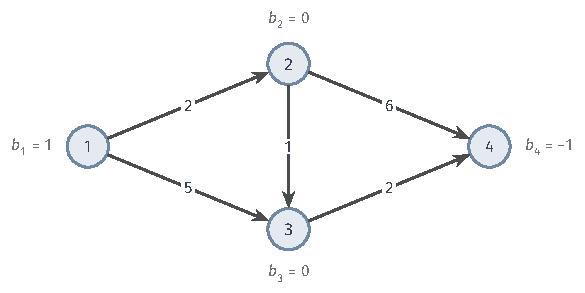
\includegraphics[width=99mm]{figures/05-optimization/01-linear-programming/tikz/lp-network-instance/figure.pdf}
 \caption{一个小网络流实例。弧旁的数字是单位费用$c_{i,j}$，节点旁的$b_i$是净供给：正数表示运出，负数表示收到，零表示只中转。每条弧上的流量$x_{i,j}\geq0$待定。}
 \label{fig:lp-network-instance}
\end{BookInlineFigure}

记弧$(i,j)$上的流量为$x_{i,j}\geq0$。每个节点都要平账：运出的总量减去运入的总量，等于该节点的净供给$b_i$，这称为流量守恒。把五条弧按$(1,2),(1,3),(2,3),(2,4),(3,4)$排列，四个守恒等式合起来就是$\bm{A}\bm{x}=\bm{b}$，其中
\begin{equation}
 \bm{A}=\begin{bmatrix}
 1&1&0&0&0\\
 -1&0&1&1&0\\
 0&-1&-1&0&1\\
 0&0&0&-1&-1
 \end{bmatrix},\qquad
 \bm{b}=\begin{bmatrix}1\\0\\0\\-1\end{bmatrix}.
 \label{eq:lp-network-data}
\end{equation}
$\bm{A}$的每一列对应一条弧，在弧的起点处为$+1$，在终点处为$-1$，其余为零，它是有向图的关联矩阵。

费用向量是$\bm{c}=(2,5,1,6,2)^\top$，总费用$\bm{c}^\top\bm{x}$是线性函数。于是最小费用的运送方案由下面的问题决定：
\[
 \min_{\bm{x}}\ \bm{c}^\top\bm{x}
 \quad\text{s.t.}\quad\bm{A}\bm{x}=\bm{b},\quad\bm{x}\geq\bm{0}.
\]
这里净供给恰好是把一单位货物从节点$1$送到节点$4$，所以问题就是求最短路。若某条弧还有容量上限$x_{i,j}\leq u_{i,j}$，只需多加一条不等式。图上这些问题的专门算法可参考\BookChapterRef{chap:min-cost-flow}{卷三第7章“最小费用流”}，本章只把它们当作线性规划的实例。

\paragraph{标准型}
比较两个模型：资源配置用“$\leq$”约束一般的线性组合，网络流用等式，只把不等号留给单个变量。第二种写法对计算更方便。一组等式可以用线性代数处理，而不等式全部成了“某个坐标非负”，这是最简单的一种不等式。我们把它定为统一的形式。

\begin{definition}[线性规划的标准型]
 \label{def:lp-standard}
 给定$\bm{A}\in\mathbb{R}^{m\times n}$、$\bm{b}\in\mathbb{R}^m$和$\bm{c}\in\mathbb{R}^n$，问题
 \begin{equation}
  \min_{\bm{x}\in\mathbb{R}^n}\ \bm{c}^\top\bm{x}
  \quad\text{s.t.}\quad\bm{A}\bm{x}=\bm{b},\quad\bm{x}\geq\bm{0}
  \label{eq:lp-standard}
 \end{equation}
 称为线性规划的\term{标准型}（standard form），它的可行集记为
 \begin{equation}
  \bm{C}=\{\bm{x}\in\mathbb{R}^n:\bm{A}\bm{x}=\bm{b},\ \bm{x}\geq\bm{0}\}.
  \label{eq:lp-feasible-set}
 \end{equation}
 $\bm{A}$的第$j$列记为$\bm{a}_j=\bm{A}_{:,j}$，最优值记为$p^\star$。
\end{definition}

可以把标准型想成一本账：每个等式是一笔必须平的账，每个变量是一项不能为负的余额。这个比喻只说明约束的形式，并不表示变量都有“余额”的含义。

\paragraph{改写成标准型}
一般的线性规划可以逐项改写。每一步都要说清新旧问题的解怎样相互对应，下面逐种列出。

\emph{最大化改为最小化。}最大化$\bm{p}^\top\bm{x}$与最小化$(-\bm{p})^\top\bm{x}$的最优解相同，最优值互为相反数。

\emph{小于等于约束。}对$\bm{g}^\top\bm{x}\leq h$，引入新变量$s=h-\bm{g}^\top\bm{x}$，约束等价于
\begin{equation}
 \bm{g}^\top\bm{x}+s=h,\qquad s\geq0.
 \label{eq:lp-slack}
\end{equation}
$s$称为\term{松弛变量}（slack variable），它是这条约束还剩的余量。

\emph{大于等于约束。}对$\bm{g}^\top\bm{x}\geq h$，减去\term{剩余变量}（surplus variable）$s=\bm{g}^\top\bm{x}-h\geq0$，得到$\bm{g}^\top\bm{x}-s=h$。

\emph{变量有上下界。}若$x_j\geq l_j$，令$x_j'=x_j-l_j\geq0$；若$x_j\leq u_j$，把它当作一条“小于等于”约束加松弛变量。

\emph{无符号限制的变量。}这样的变量称为\term{自由变量}（free variable）。把它写成两个非负变量之差：
\begin{equation}
 x_j=x_j^{+}-x_j^{-},\qquad x_j^{+}\geq0,\quad x_j^{-}\geq0.
 \label{eq:lp-free-split}
\end{equation}

\begin{example}[车间问题的标准型]
 \label{ex:lp-workshop-standard}
 为工时和原料分别引入松弛变量$x_3,x_4\geq0$，把最大化利润改成最小化利润的相反数，就得到$n=4$，$m=2$的标准型，数据是
 \begin{equation}
  \bm{A}=\begin{bmatrix}1&1&1&0\\2&1&0&1\end{bmatrix},\quad
  \bm{b}=\begin{bmatrix}4\\6\end{bmatrix},\quad
  \bm{c}=\begin{bmatrix}-3\\-2\\0\\0\end{bmatrix}.
  \label{eq:lp-workshop-standard}
 \end{equation}
 第~\ref{chap:optimization}章的解$(x_1,x_2)=(2,2)$对应$\bm{x}=(2,2,0,0)^\top$，工时和原料都恰好用完，目标值是$-10$。
\end{example}

松弛变量的意义可以直接在图上读出。图~\ref{fig:lp-slack-meaning}中，取产量$(1,1)$，代入得到
\[
 x_3=4-1-1=2,\qquad x_4=6-2-1=3.
\]
也就是工时还剩$2$，原料还剩$3$。$x_3=0$恰好是工时约束的边界，$x_3=2$是与边界平行的另一条直线。平面上每个点都对应一组松弛变量的值，点走到哪条边界上，对应的松弛变量就降为零。

\begin{BookInlineFigure}
 \centering
 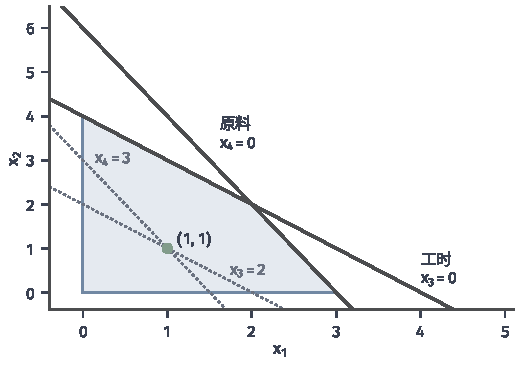
\includegraphics[width=88mm]{figures/05-optimization/01-linear-programming/matplotlib/lp-slack-meaning/figure.pdf}
 \caption{车间问题的松弛变量。深灰粗线是约束取等号的边界，也就是$x_3=0$和$x_4=0$。过绿点$(1,1)$的两条灰色点线是与边界平行的直线，在它们上面$x_3=2$，$x_4=3$，表示这一产量剩下的工时和原料。}
 \label{fig:lp-slack-meaning}
\end{BookInlineFigure}

\paragraph{改写保留了什么}
松弛变量的引入是一一对应的。原问题的可行点$\bm{x}$对应新问题的可行点$(\bm{x},\bm{b}-\bm{A}\bm{x})$，反过来，丢掉松弛变量就回到原来的点。目标值不变，因为松弛变量的费用是零。这个对应是仿射映射，保持线段和中点，所以可行集的形状也保留下来：车间的四边形搬进了$\mathbb{R}^4$，还是同一个四边形。

自由变量的分解不同。从分解后的可行点总能算出原来的$x_j$，目标值相同，所以最优值和最优解的集合不变。但同一个$x_j$有无穷多种写法，图~\ref{fig:lp-free-split}中$(x^{+},x^{-})=(1,0)$和$(3,2)$都表示$x=1$。

\begin{BookInlineFigure}
 \centering
 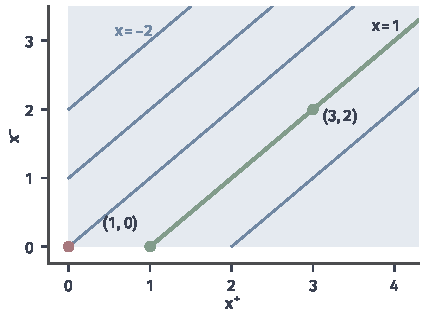
\includegraphics[width=72mm]{figures/05-optimization/01-linear-programming/matplotlib/lp-free-split/figure.pdf}
 \caption{自由变量的分解$x=x^{+}-x^{-}$。浅蓝区域是分解后允许的第一象限，每条斜线上的点代表同一个$x$，绿色粗线是$x=1$。原来的直线变成了一个象限，红点$(0,0)$是这个象限唯一的角点，它在原来的直线上只是普通的一点$x=0$。}
 \label{fig:lp-free-split}
\end{BookInlineFigure}

分解后新问题的最优解可能不唯一，例如沿斜线同时增大$x^{+}$和$x^{-}$，目标值不变。分解还会凭空造出角点：实数轴没有角，第一象限却有角点$(0,0)$。下一节谈顶点时要记住这一点。表~\ref{tab:lp-transformations}汇总了各种改写的效果。

\begin{BookInlineTable}
 \centering
 \begin{tabular}{lll}
  \toprule
  改写 & 解的对应 & 变化 \\
  \midrule
  最大改最小 & 最优解相同 & 最优值变号 \\
  加松弛或剩余变量 & 一一对应 & 变量增加，形状不变 \\
  变量平移 & 一一对应 & 平移可行集 \\
  自由变量分解 & 多对一 & 可能多出角点和最优解 \\
  \bottomrule
 \end{tabular}
 \caption{改写成标准型时各步保留的内容。每一步都保持最优值（或只差符号与常数），并且可以从新问题的解算出原问题的解。}
 \label{tab:lp-transformations}
\end{BookInlineTable}

\paragraph{冗余等式与满行秩}
下一节要从$\bm{A}$中选出可逆的方阵，这需要$\bm{A}$的行没有多余。网络流的矩阵~\eqref{eq:lp-network-data}就有多余的行：每一列恰有一个$+1$和一个$-1$，所以四行相加是零向量，第四行是前三行之和的相反数。$\bm{b}$的分量相加也是零，这说明总供给等于总需求，等式组是相容的。

一般的处理分两步。先检查等式组是否相容，也就是比较$\operatorname{rank}\bm{A}$和增广矩阵的秩：
\[
 \operatorname{rank}\bm{A}=\operatorname{rank}\bigl[\bm{A}\ \ \bm{b}\bigr].
\]
若上式不成立，等式组无解，可行集是空集，问题到此回答完毕。在网络中这对应总供给不等于总需求，货物无处可去。

若相容且$\operatorname{rank}\bm{A}=r<m$，就选出$r$个线性无关的行，其余的行是它们的线性组合，右端也是相应的组合，删去后解集不变。网络的例子里删去第四行即可，剩下三行线性无关，这只要看弧$(1,2),(2,3),(3,4)$三列组成的$3\times3$子矩阵，它是可逆的三角矩阵。秩判别和选主元消元的做法可参考\BookChapterRef{chap:linear-solution-selection}{卷二第11章“线性方程与最小二乘的选解”}。

以后凡涉及基矩阵，都假设已完成这一步，即
\begin{equation}
 \operatorname{rank}\bm{A}=m\leq n.
 \label{eq:lp-full-row-rank}
\end{equation}
车间问题的$\bm{A}$含有单位矩阵，自动满行秩。
